\documentclass{article}

% Language setting
% Replace `english' with e.g. `spanish' to change the document language
\usepackage[french]{babel}
\usepackage{amsmath}
\usepackage{stmaryrd}
\usepackage{comment}
\usepackage[final]{graphicx}

%\usepackage{natbib}
\usepackage[numbers]{natbib}


% Set page size and margins
% Replace `letterpaper' with`a4paper' for UK/EU standard size
\usepackage[letterpaper,top=2cm,bottom=2cm,left=3cm,right=3cm,marginparwidth=1.75cm]{geometry}

% Useful packages
\usepackage{amsmath}
\usepackage{graphicx}
\usepackage[colorlinks=true, allcolors=blue]{hyperref}

\DeclareMathOperator*{\argmax}{argmax}

\title{Responsible Machine learning - Final technical assignment}
\author{Abdellah Elmrini \and Jérémie Dentan \and Nathanaël Cuvelle--Magar}

\begin{document}
\maketitle

\section*{Introduction}

\begin{comment}
    Now state of the art in many fields, deep learning algorithms have revolutionised the way we approach many tasks, particularly in computer vision \cite{He2015DelvingDI}.
Nevertheless, these excellent performances are offset by certain weaknesses, foremost among which is the vulnerability to adversarial attacks. Highlighted in numerous papers \cite{Kurakin2016AdversarialML,Goodfellow2014ExplainingAH}, they usually exploit the fact that the reasons for a classifier to predict a certain outcome are not those perceived by human analysts \footnote{In this project, we will focus on evasion attacks and will not address the issue of poisoning attacks.}. An imperceptible change in an image can thus lead to a completely wrong classification, as illustrated by \citet{Goodfellow2014ExplainingAH} (FGSM, for Fast Gradient Sign Attack). This vulnerability is thus a major problem for anyone wishing to use a DNN in security-critical systems. However, attacks such as FGSM require knowledge of the architecture and weights of the network to be attacked, and therefore impose a white box setting. The existence of black box attacks, which do not require knowledge of the target model and its weights, therefore represents an important security issue, which has led to the development of a research field dedicated to the transferability of attacks \cite{Liu2016DelvingIT}. From sound \cite{Subramanian2019RobustnessOA, Subramanian2020ASO} to text \cite{Yuan2020OnTT} and computer vision \cite{Naseer2019CrossDomainTO}, the objective is to design adversarial examples from a generating model to fool a target model. \citet{Demontis2018WhyDA} highlight several criteria influencing the performance of these attacks, including the simplicity of the generating model. Based on the fact that neural networks trained on large image datasets learn generic internal representations that are transferable to new tasks and datasets, \citet{Naseer2018TaskgeneralizableAA} propose to use a perceptual metric based on VGG internal representations to design transferable attacks. The authors thus implicitly use the Natural Abstraction Hypothesis, according to which 'a wide variety of cognitive architectures will learn to use approximately the same high-level abstract objects/concepts to reason about the world' \cite{NatAbsHyp}.\\
Our goal in this project is to implement the attack proposed by \citet{Naseer2018TaskgeneralizableAA} 
\end{comment}

Aujourd'hui à l'état de l'art dans de nombreux domaines, les algorithmes de \textit{deep learning} (DL) ont révolutionné notre façon d'aborder de nombreuses tâches, en particulier en \textit{computer vision} \cite{He2015DelvingDI}.
Néanmoins, ces excellentes performances sont contrebalancées par certaines fragilités, au premier rang desquelles la vulnérabilité aux attaques adversariales. Mises en évidence dans de nombreux articles \cite{Kurakin2016AdversarialML,Goodfellow2014ExplainingAH}, elles exploitent généralement le fait que les raisons poussant un classifieur à prédire un certain résultat ne sont pas celles perçues par les analystes humains \footnote{Dans ce projet, nous nous concentrerons sur les \textit{evasion attacks} et n'aborderons pas la question des \textit{poisoning attacks}.}. Une modification imperceptible d'une image peut ainsi conduire à une classification complètement erronée, comme illustré par \citet{Goodfellow2014ExplainingAH} (FGSM, pour \textit{Fast Gradient Sign Attack}). Cette vulnérabilité est ainsi un problème majeur pour quiconque souhaite utiliser un \textit{deep neural network} (DNN) dans un système sécurisé. Malgré tout, des attaques comme FGSM nécessitent de connaître l'architecture et les poids du réseau que l'on souhaite attaquer, et imposent donc une configuration \textit{white box}. L'existence d'attaques \textit{black box}, ne nécessitant pas de connaître le modèle cible et ses poids, représente donc un enjeu de sécurité important, qui a conduit au développement d'un champ de recherche dédié à la transférabilité des attaques \cite{Liu2016DelvingIT}. Du son \cite{Subramanian2019RobustnessOA, Subramanian2020ASO} au texte \cite{Yuan2020OnTT} en passant par la \textit{computer vision} \cite{Naseer2019CrossDomainTO}, l'objectif est de concevoir des exemples adversariaux à partir d'un modèle de génération pour tromper un modèle cible. \citet{Demontis2018WhyDA} mettent en évidence plusieurs critères influençant les performances de ces attaques, dont la simplicité du modèle générateur. S'appuyant sur le fait que les DNNs entraînés sur de grands jeux de données apprennent des représentations internes génériques transférables à de nouvelles tâches et à de nouveaux jeux de données, \citet{Naseer2018TaskgeneralizableAA} proposent d'utiliser une métrique perceptuelle fondée sur les représentations internes des réseaux VGG pour concevoir des attaques transférables. Les auteurs utilisent ainsi implicitement la \textit{Natural Abstraction Hypothesis}, selon laquelle "une grande variété d'architectures cognitives vont apprendre à utiliser approximativement les mêmes objets/concepts abstraits de haut niveau pour raisonner sur le monde" \cite{NatAbsHyp}. \\

\noindent Notre but dans ce projet est d'implémenter l'attaque proposée par \citet{Naseer2018TaskgeneralizableAA} et de la confronter aux résultats généraux sur la transférabilité des attaques proposées par \citet{Demontis2018WhyDA}. En s'appuyant sur les résultats de ce dernier papier, nous chercherons également, dans un second temps, à établir si un processus de génération plus robuste pour les exemples adversariaux peut permettre d'améliorer leur transférabilité au-delà de la complexité du modèle de génération choisi. \\

\noindent Ce rapport est accompagné d'un répertoire Github qui en implémente les principales expérimentations, disponible à l'addresse suivante: \url{https://github.com/DentanJeremie/adversarialTransferts}.

\begin{comment}
Sur la transférabilité en vision \cite{Naseer2018TaskgeneralizableAA, Naseer2019CrossDomainTO}, en NLP \cite{Yuan2020OnTT}, pour les sons \cite{Subramanian2020ASO}, sur la robustesse \cite{Subramanian2019RobustnessOA}, sur la compréhension de la transférabilité \cite{Demontis2018WhyDA}. Article beaucoup cité \cite{Liu2016DelvingIT}. Sur la superposition et le lien avec les attaques \cite{Elhage2022ToyMO}. Idée globale : Natural Abstraction Hypothesis $\longrightarrow$ circuits universaux $\longrightarrow$ attaques transférables (non spécifiques à un domaine ou à un modèle). Sujet possible : les articles implémentant des attaques transférables ne reposent-ils pas, en réalité, sur l'attaque des circuits universaux (bien qu'ils ne le mentionnent pas) ?
\end{comment}

\section{Transférabilité via des métriques perceptuelles}
\label{chap:transferability_perceptual}

Dans cette partie, on cherche à évaluer la transférabilité de l'attaque NRDM, pour \textit{Neural Representation Distortion Method}, proposée par \citet{Naseer2018TaskgeneralizableAA} et à vérifier l'applicabilité des résultats de \citet{Demontis2018WhyDA} dans ce cadre.

\subsection{Rappels sur la transférabilité des attaques}

Comme évoqué en introduction, \citet{Naseer2018TaskgeneralizableAA} utilisent une métrique perceptuelle pour créer des attaques dont la transférabilité repose sur la générécité des représentations apprises par les \textit{neural networks} (NNs) lorsqu'ils sont entraînés sur de grands jeux de données, comme ImageNet \cite{Russakovsky2014ImageNetLS}. Plus précisément, les auteurs proposent de concevoir les exemples adversariaux de la façon suivante : $$\argmax\limits_{x'} \left\{\mathcal{F}(x')|_k - \mathcal{F}(x)|_k \quad / \quad ||x-x'||_{\infty} \le \epsilon \right\},$$
où $\mathcal{F}$ est un NN générateur, $k$ est l'indice d'une couche, $\mathcal{F}(x)|_k$ désigne l'évaluation de $\mathcal{F}$ tronqué à la couche $k$ en $x$, et $\epsilon$ est le budget de perturbation autorisé. L'idée est ainsi de chercher l'image d'entrée dont la représentation interne de niveau $k$ diffère le plus de celle de l'image d'origine, à budget de perturbation fixé. Une description détaillée de l'algorithme utilisé est donnée dans l'article original. Nous en proposons une implémentation disponible sur GitHub \footnote{\url{https://github.com/DentanJeremie/adversarialTransferts}}, utilisant VGG16 \cite{Simonyan2014VeryDC} comme modèle générateur (pré-entraîné sur ImageNet). La figure \ref{fig:NRDM} illustre les résultats obtenus sur le jeu de données Tiny ImageNet \cite{Le2015TinyIV}, avec $5$ étapes de descente de gradient, $\epsilon = 16/256$ et $k$ correspondant à la couche "conv33".\\

\begin{figure}
\centering
\subfloat{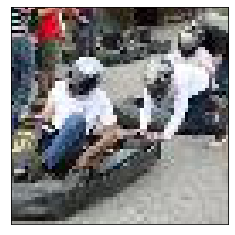
\includegraphics[width = 1in]{tiny_imnet_0.png}}
\subfloat{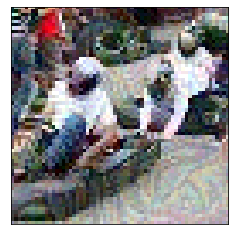
\includegraphics[width = 1in]{tiny_imnet_0_adv.png}}
\subfloat{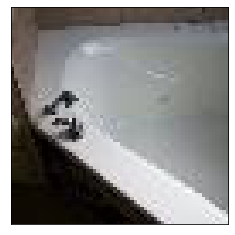
\includegraphics[width = 1in]{tiny_imnet_3.png}}
\subfloat{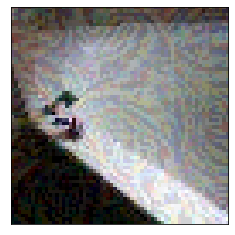
\includegraphics[width = 1in]{tiny_imnet_3_adv.png}}\\
\subfloat{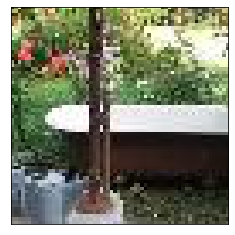
\includegraphics[width = 1in]{tiny_imnet_4.png}}
\subfloat{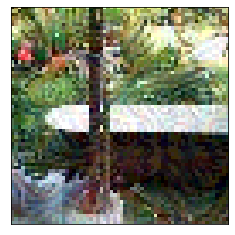
\includegraphics[width = 1in]{tiny_imnet_4_adv.png}}
\subfloat{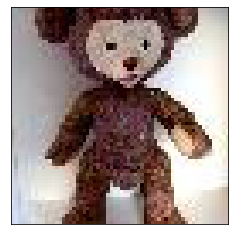
\includegraphics[width = 1in]{tiny_imnet_5.png}}
\subfloat{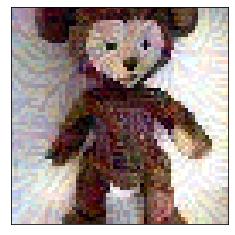
\includegraphics[width = 1in]{tiny_imnet_5_adv.png}}\\
\subfloat{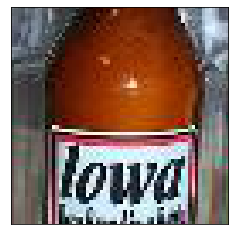
\includegraphics[width = 1in]{tiny_imnet_7.png}}
\subfloat{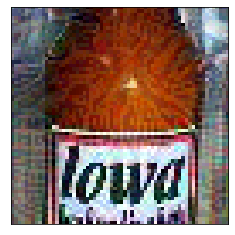
\includegraphics[width = 1in]{tiny_imnet_7_adv.png}}
\subfloat{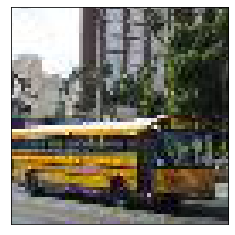
\includegraphics[width = 1in]{tiny_imnet_8.png}}
\subfloat{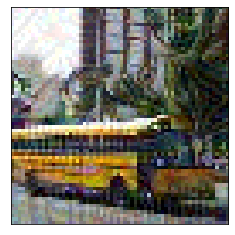
\includegraphics[width = 1in]{tiny_imnet_8_adv.png}}
\caption{Exemples d'images adversariales perceptuelles.}
\label{fig:NRDM}
\end{figure}

\noindent De leur côté, \citet{Demontis2018WhyDA} étudient les facteurs favorisant la transférabilité des attaques. Ils en identifient trois principaux :
\begin{itemize}
    \item la taille des gradients d'entrée, qui est liée à la complexité du modèle cible, puisque les classifieurs cibles complexes tendent à présenter des gradients plus importants ;
    \item l'alignement des gradients des modèles générateurs et cibles, qui est, pour les \textit{evasion attacks}, lié à la complexité du générateur, puisque des générateurs de faibles complexités donnent des gradients plus stables et mieux alignés, en moyenne, avec ceux de la cible ;
    \item la variabilité du paysage de la fonction de perte.
\end{itemize}

\subsection{Evaluation des attaques perceptuelles}

Les résultats de \citet{Demontis2018WhyDA} ayant été obtenus pour une tâche de classification binaire et pour des algorithmes d'apprentissage variés, i.e. pas uniquement des NNs (SVM, logistic regression, etc.) \footnote{Les auteurs ne distinguent pas réellement entre les architectures. Notre objectif est donc de voir si leurs résultats sont toujours valables si l'on compare des algorithmes de type NN entre eux.}, nous souhaitons voir s'ils restent valables dans le contexte de l'attaque proposée par \citet{Naseer2018TaskgeneralizableAA}. Plus particulièrement, nous souhaitons voir si les facteurs proposés peuvent être reliés au choix de la couche d'index $k$ dans NRDM, cette dernière contrôlant en un sens la complexité du modèle de génération. Nous chercherons également à voir si l'efficacité de cette attaque dépend du nombre de paramètre du NN cible, utilisé comme un proxy de sa complexité. Enfin, nous évaluerons l'impact du nombre d'étapes de descente de gradients réalisées sur l'efficacité des exemples adversariaux produits.\\
Les résultats obtenus sont donnés dans les tableaux \ref{table:VGG_accuracy} (target VGG16), \ref{table:DenseNet_accuracy} (target DenseNet201 \cite{Huang2016DenselyCC}) et \ref{table:ResNet_accuracy} (target ResNet50 \cite{He2015DeepRL}). Dans toutes ces expériences, $\epsilon$ est fixé à $16/256$.

\begin{table}[!h]
\centering
\caption{VGG \textit{accuracy} sur les données corrompues (performances initiales 0.4042)}
\label{table:VGG_accuracy}
\begin{tabular}{|c|l|l|l|l|}
\hline
Attaque      & \multicolumn{1}{c|}{3 étapes} & \multicolumn{1}{c|}{5 étapes} & 7 étapes & 10 étapes \\ \hline
vgg\_conv22 & 0.1376                       & 0.1060                       & 0.0964  & 0.0937   \\ \hline
vgg\_conv33 & 0.0704                       & 0.0475                       & 0.0420  & 0.0412   \\ \hline
vgg\_conv43 & 0.0444                       & 0.0341                       & 0.0296  & 0.0288   \\ \hline
\end{tabular}
\end{table}

\begin{table}[!h]
\centering
\caption{DenseNet \textit{accuracy} sur les données corrompues (performances initiales 0.6489)}
\label{table:DenseNet_accuracy}
\begin{tabular}{|c|l|l|l|l|}
\hline
Attaque      & \multicolumn{1}{c|}{3 étapes} & \multicolumn{1}{c|}{5 étapes} & 7 étapes & 10 étapes \\ \hline
vgg\_conv22 & 0.2558                       & 0.2518                       & 0.2458  & 0.2398   \\ \hline
vgg\_conv33 & 0.2347                       & 0.2107                       & 0.2047  & 0.1964   \\ \hline
vgg\_conv43 & 0.2297                       & 0.2086                       & 0.2090  & 0.2037   \\ \hline
\end{tabular}
\end{table}

\begin{table}[!h]
\centering
\caption{ResNet \textit{accuracy} sur les données corrompues (performances initiales 0.7354)}
\label{table:ResNet_accuracy}
\begin{tabular}{|c|l|l|l|l|}
\hline
Attaque      & \multicolumn{1}{c|}{3 étapes} & \multicolumn{1}{c|}{5 étapes} & 7 étapes & 10 étapes \\ \hline
vgg\_conv22 & 0.2768                       & 0.2565                       & 0.2447  & 0.2378   \\ \hline
vgg\_conv33 & 0.2548                       & 0.2218                       & 0.2107  & 0.2105   \\ \hline
vgg\_conv43 & 0.2363                       & 0.2184                       & 0.2170  & 0.2106   \\ \hline
\end{tabular}
\end{table}

\noindent On fait les observations suivantes :
\begin{itemize}
    \item L'augmentation du nombre d'itération de la descente de gradient améliore presque toujours les performances de l'attaque. Néanmoins, on observe que son impact finit par se tasser.
    \item L'impact de la complexité du modèle générateur varie suivant le nombre d'étapes de \textit{gradient descent} (GD) réalisées et il faut donc distinguer les cas. Lorsque ce nombre est faible ($3,5$), il apparaît qu'une attaque fondée sur une couche plus élevée fonctionne mieux quel que soit le modèle cible. On peut l'interpréter en considérant que, si l'on tronque le réseau trop bas, les perturbations obtenues dépendront trop du réseau en question. Contrairement à ce qui se passe quand on tronque à une couche supérieure, ce ne seront pas des "\textit{high level features}". Ce  constat semble aller à l'encontre du principe de simplicité pour le modèle générateur. Néanmoins, on observe que pour un nombre d'étapes de GD plus important ($7,10$), cette dynamique n'est plus celle obtenue pour les modèles DenseNet201 et ResNet50. En effet, on observe alors un optimum pour une attaque basée sur la couche de profondeur intermédiaire "vgg\_conv33", indiquant peut être un compromis entre "\textit{high level features}" et faible complexité du générateur. Le cas où VGG16 est le modèle cible correspond quant à lui à un cas particulier, puisqu'augmenter l'index $k$ conduit à rapprocher le modèle générateur du modèle cible. Il semble donc logique de ne pas observer le même comportement dans cette configuration.
    \item L'impact de la complexité du modèle cible semble être confirmé. En effet, les modèles VGG16, DenseNet201 et ResNet50 présentent, respectivement, 138357544, 20013928 et 25557032 paramètres, et on vérifie que les performances de l'attaque NRDM sont d'autant plus importantes que le modèle a de paramètres. Pour quantifier ces performances, on considère le ratio entre les performances originales du modèle et celles obtenues pour la meilleure configuration d'attaque. Pour DenseNet201 et ResNet50, cela revient à considérer $10$ d'étapes de GD et la couche "vgg\_conv33" pour la génération. Pour VGG16, on considère la même configuration afin de permettre une comparaison équitable. En effet, comme évoqué plus haut, les meilleures performances obtenues pour des couches plus élevées sont à relier au fait que VGG est le modèle générateur. On obtient les résultats suivants : $3.30$ pour DenseNet201, $3.49$ pour ResNet50 et $9.81$ pour VGG16.
\end{itemize}
Par conséquent, nos résultats semblent aller dans le sens de ceux obtenus par \citet{Demontis2018WhyDA}. Il pourrait notamment être intéressant de vérifier le rapport entre nombre de paramètres du modèle cible et la performance maximale de l'attaque NRDM qui semble, pour les modèles considérés ici, linéaire. Nous laissons cette vérification à de prochains travaux.

\section{Conception robuste des exemples adversariaux}

La partie précédente a permis de confirmer, dans une certaine mesure, les résultats de \citet{Demontis2018WhyDA} quant à l'importance de la simplicité du modèle de génération pour les exemples adversariaux. On note néanmoins que la méthode utilisée pour les construire repose sur une descente gradient classique, correspondant à une métrique $L^2$. Or, des travaux réalisés dans le domaine de la visualisation des \textit{features} montrent qu'un tel processus d'optimisation peut se révéler sensible aux hautes fréquences, tandis qu'une paramétrisation Fourier/décorrélée permet de réduire leur impact \cite{FeatVizualize}. Par suite, nous proposons dans cette partie d'implémenter l'attaque NRDM avec une telle paramétrisation en s'appuyant sur la librairie PyTorch Lucent \footnote{\url{https://github.com/greentfrapp/lucent}}. L'idée est de réduire la complexité des exemples adversariaux, d'une façon complémentaire à celle du modèle de génération.\\

\noindent On commence par illustrer la différence entre les perturbations obtenues suivant la paramétrisation adoptée. On considère les images d'entrée présentées en figure \ref{fig:input_FFT_decorrelated}.

\begin{figure}[!h]

      \begin{minipage}[b]{0.4\linewidth}
       \centering
       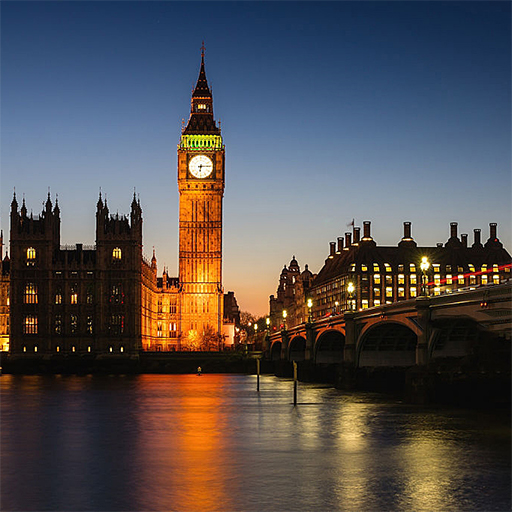
\includegraphics[width = \linewidth]{img_b.png}     
      \end{minipage}
    \hfill
      \begin{minipage}[b]{0.375\linewidth}
       \centering
       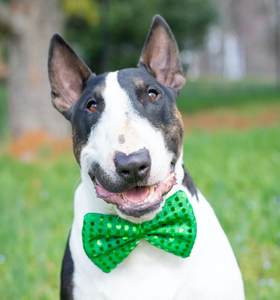
\includegraphics[width = \linewidth]{dog.png}     
      \end{minipage}
      \caption{Images d'entrée utilisées pour illustrer l'impact du choix de paramétrisation.}
      \label{fig:input_FFT_decorrelated}
    
    \end{figure}

\noindent On considère deux configurations :
\begin{itemize}
    \item Pour la première image, représentant le Big Ben, dont l'état d'origine est présenté sur la figure \ref{fig:input_FFT_decorrelated} (gauche) et les perturbations sur la figure \ref{fig:BigBen_pertubation}, on utilise le modèle Inceptionv1 et on maximise la \textit{Mean Squared Error} entre les \textit{features} obtenus en sortie de la couche "mixed3b" pour l'image d'origine et l'image paramétrée. Cette dernière est initialisée à la valeur de l'image d'origine, sans bruit additionnel. $10$ étapes de GD sont calculées (l'image perturbée obtenue n'est pas clippée, l'objectif étant ici purement illustratif). Les résultats pour les paramétrisations classiques (gauche) et Fourier/décorrélées (droite) sont illustrés en figure \ref{fig:BigBen_pertubation}.
    \item Pour la seconde image, représentant un chien, dont l'état d'origine est présenté sur la figure \ref{fig:input_FFT_decorrelated} (droite) et les perturbations sur la figure \ref{fig:dog_perturbation}, on utilise le modèle VGG16 et on maximise la \textit{Mean Squared Error} entre les \textit{features} obtenus en sortie de la couche "features\_30" (dernière couche avant le classifieur) pour l'image d'origine et l'image paramétrée. Cette dernière est initialisée à la valeur de l'image d'origine, avec un bruit additionnel gaussien d'amplitude $\epsilon = 16/256$. $1$ (gauche), $10$ (milieu) et $100$ (droite) étapes de GD sont calculées (l'image perturbée obtenue n'est pas clippée, l'objectif étant ici purement illustratif). Les résultats pour les paramétrisations classiques (haut) et Fourier/décorrélées (bas) sont illustrés en figure \ref{fig:dog_perturbation}.
\end{itemize}

\begin{figure}[!h]

      \begin{minipage}[b]{0.4\linewidth}
       \centering
       
\includegraphics[width = \linewidth]{img_b_l2_b.png}     
      \end{minipage}
    \hfill
      \begin{minipage}[b]{0.4\linewidth}
       \centering
       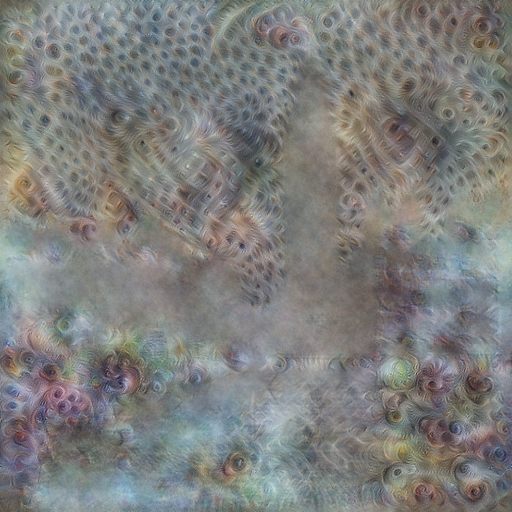
\includegraphics[width = \linewidth]{img_b_fft_b.png}     
      \end{minipage}
      \caption{Perturbation (i.e. image perturbée moins image d'origine) pour la figure \ref{fig:input_FFT_decorrelated} (gauche).}
      \label{fig:BigBen_pertubation}
    
    \end{figure}

\begin{figure}[!h]
\centering
\subfloat{
\includegraphics[width = 1.5in]{dog_1.png}}
\subfloat{
\includegraphics[width = 1.5in]{dog_10.png}}
\subfloat{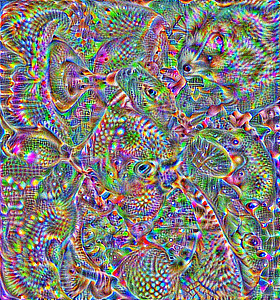
\includegraphics[width = 1.5in]{dog_100.png}}\\
\subfloat{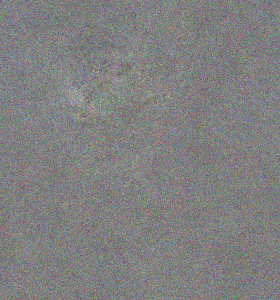
\includegraphics[width = 1.5in]{dog_fft_decorrelate_1.png}}
\subfloat{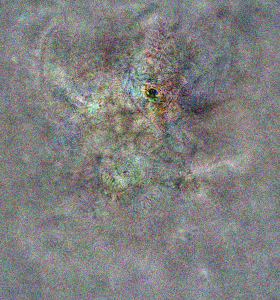
\includegraphics[width = 1.5in]{dog_fft_decorrelate_10.png}}
\subfloat{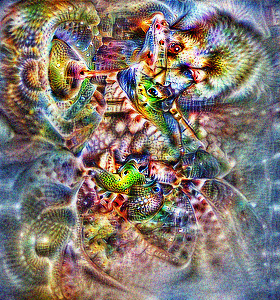
\includegraphics[width = 1.5in]{dog_fft_decorrelate_100.png}}
\caption{Perturbation (i.e. image perturbée moins image d'origine) pour la figure \ref{fig:input_FFT_decorrelated} (droite).}
\label{fig:dog_perturbation}
\end{figure}

\noindent En accord avec les résultats présentés dans \cite{FeatVizualize}, on observe qu'une optimisation dans l'espace Fourier/décorrélé semble, d'une part, mieux retranscrire la structure de l'image et, d'autre part, réduire l'impact des hautes fréquences.\\% On illustre en figure \ref{fig:corrupted_img} les images corrompues obtenues pour les entrées de la figure \ref{fig:input_FFT_decorrelated}.\\
\begin{comment}
    
\begin{figure}[!h]

      \begin{minipage}[b]{0.4\linewidth}
       \centering
       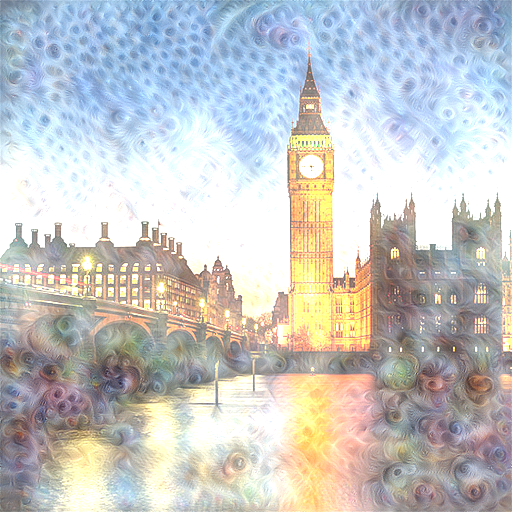
\includegraphics[width = \linewidth]{img_b_img.png}     
      \end{minipage}
    \hfill
      \begin{minipage}[b]{0.375\linewidth}
       \centering
       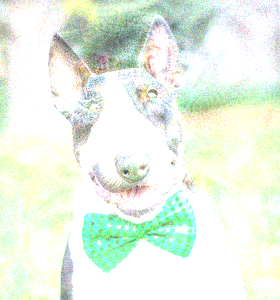
\includegraphics[width = \linewidth]{dog_fft_decorrelate_10_img.png}     
      \end{minipage}
      \caption{Images corrompues obtenues pour les entrées de la figure \ref{fig:input_FFT_decorrelated}.}
      \label{fig:corrupted_img}
    
    \end{figure}
\end{comment}

\noindent De la même façon qu'en partie \ref{chap:transferability_perceptual}, on compare les performances obtenues avec ces deux versions de NRDM. Les résultats sont les suivants, pour DenseNet201 (resp. ResNet50) en modèle cible : 0.5782 (resp. 0.6230) pour une paramétrisation classique et 0.5846 (resp. 0.6549) pour une paramétrisation Fourier/décorrélée \footnote{Ces valeurs sont calculées pour un échantillon de $300$ exemples adversariaux avec VGG16 comme modèle génératif, en sélectionnant la couche 5 du réseau et pour $100$ étapes de GD. $\epsilon$ est toujours fixé à $16/256$.}. On n'observe donc pas d'amélioration significative des performances de l'attaque lorsque la seconde est utilisée, ce qui semble suggérer qu'une optimisation limitant l'impact des hautes fréquences n'est pas directement reliée à la réduction de complexité préconisée par \citet{Demontis2018WhyDA}.\\
À titre de complément, les tableaux \ref{tab:DenseNet_accuracy_fft_dec} et \ref{tab:ResNet_accuracy_fft_dec} présentent les résultats obtenus dans diverses configurations de l'attaque avec paramétrisation Fourier/décorrélée. On note que, dans ce cadre, les attaques généralisent d'autant mieux qu'elles ont été générées via des couches peu profondes.

\begin{table}[!h]
\centering
\caption{DenseNet \textit{accuracy} sur les données corrompues (performances initiales 0.66)}
\label{tab:DenseNet_accuracy_fft_dec}
\begin{tabular}{|c|l|l|}
\hline
Attaque      & \multicolumn{1}{c|}{100 étapes} & \multicolumn{1}{c|}{250 étapes}  \\ \hline
vgg, couche 5 & 0.5846                      & 0.4632                    \\ \hline
vgg, couche 7& 0.6130                   & 0.5367                   \\ \hline
\end{tabular}
\end{table}

\begin{table}[!h]
\centering
\caption{ResNet \textit{accuracy} sur les données corrompues (performances initiales 0.73)}
\label{tab:ResNet_accuracy_fft_dec}
\begin{tabular}{|c|l|l|}
\hline
Attaque      & \multicolumn{1}{c|}{100 étapes} & \multicolumn{1}{c|}{250 étapes}  \\ \hline
vgg, couche 5 & 0.6549                      & 0.5623                    \\ \hline
vgg, couche 7& 0.7093                   & 0.5879                   \\ \hline
\end{tabular}
\end{table}

\section*{Conclusion}

En résumé, il apparaît que les résultats de \citet{Demontis2018WhyDA} restent, dans une certaine mesure, valables dans le cadre de l'attaque NRDM et, plus généralement, dans celui où le générateur et la cible sont des NNs. L'analyse de la transférabilité des exemples adversariaux obtenus nous a notamment permis de mettre en évidence un compromis entre, d'une part, l'importance de considérer des \textit{features} d'assez haut niveau, non spécifiques au modèle, et, d'autre part, la nécessité de limiter le nombre de paramètres (i.e. la complexité) du modèle générateur (i.e. l'indice $k$).\\
L'étude de ce critère de complexité du générateur nous a également permis de considérer une voie alternative pour sa réduction, pour un nombre de paramètres fixé, en modifiant la paramétrisation de l'image perturbée pour passer dans l'espace de Fourier/décorrélé. Bien que l'impact des hautes fréquences ait ainsi pu être contenu par rapport à une descente de gradient $L^2$ classique, notre étude ne nous a pas permis de conclure qu'une telle approche puisse mener à une réelle amélioration dans la transférabilité de l'attaque.\\

\noindent Dans la continuité de ce projet et de cet approfondissement du critère de simplicité du générateur, il serait intéressant de creuser plus avant la question de la complexité du modèle cible. Pour cela, il pourrait notamment être pertinent d'étudier ses liens avec la notion de superposition dans les réseaux de neurones et ses conséquences sur la vulnérabilité aux attaques adversariales \cite{Elhage2022ToyMO}. En effet, dans les deux cas, il apparaît que la vulnérabilité aux attaques est liée à une forme de complexité du modèle, que ce soit sous la forme d'un nombre important de paramètres dans \citet{Demontis2018WhyDA}, ou d'une forte superposition des \textit{features} dans \citet{Elhage2022ToyMO}. Une expérience pour réaliser cette comparaison pourrait, par exemple, consister à construire un jeu de données d'images simples (ex. formes géométriques simples de couleurs variables) permettant d'identifier les \textit{features} appris par le réseau (forme, couleur), de façon à pouvoir ensuite établir si l'optimisation du critère perceptuel de NRDM revient effectivement à utiliser la superposition pour tromper le modèle cible. Nous laissons ces perspectives à de prochains travaux.

\bibliographystyle{plainnat}
\bibliography{sample}


\end{document}